% \documentclass{} is the first command in any LaTeX code.  
% It is used to define what kind of document you are creating 
% such as an article or a book, and begins the document preamble
\documentclass{article} 

% Set the space between paragraphs
\setlength{\parskip}{1em}

% Packages for customizing the ToC
\usepackage{tocloft}
\usepackage{xcolor} % Package for color definitions
\usepackage{hyperref}

% Create trees
\usepackage{forest}

% Create two column content
\usepackage{multicol}

% Put blocks at their specific place using [H]
\usepackage{float}

\usepackage{algorithm}% http://ctan.org/pkg/algorithms
\usepackage{algpseudocode}% http://ctan.org/pkg/algorithmicx

\usepackage{amsmath}

% Create plots
\usepackage{pgfplots}
\pgfplotsset{compat=1.17}

% Use charts with axis that are strings instead of number
\usepackage{pgfplotstable}

% For better looking tables
\usepackage{booktabs} 

% Add dots to the table of contents
\renewcommand{\cftsecleader}{\cftdotfill{\cftdotsep}}
\renewcommand{\cftsubsecleader}{\cftdotfill{\cftdotsep}}
\renewcommand{\cftsubsubsecleader}{\cftdotfill{\cftdotsep}}

% Define custom colors using xcolor
\definecolor{green400}{HTML}{4ade80}
\definecolor{green500}{HTML}{22c55e}
\definecolor{green600}{HTML}{16a34a}
\definecolor{blue400}{HTML}{60a5fa}
\definecolor{blue500}{HTML}{3b82f6}
\definecolor{blue600}{HTML}{2563eb}
\definecolor{blue700}{HTML}{1d4ed8}
\definecolor{violet600}{HTML}{8b5cf6}
\definecolor{violet400}{HTML}{a78bfa}

% Hyperlink settings
\hypersetup{
    % Enable colored links
    colorlinks=true,
    % Color for internal links (sections, pages, etc.)
    linkcolor=blue700,
    % Color for external URLs
    urlcolor=blue600,
    % Color for citation links
    citecolor=blue700
}

% Bibliography package
\usepackage[backend=biber,style=numeric]{biblatex}
\addbibresource{references.bib}

% Article title
\title{LeanIMT: An optimized Incremental Merkle Tree} 
% Authors name
\author{Privacy \& Scaling Explorations} 
% Date for date compiled
\date{\today} 

% The preamble ends with the command \begin{document}
% All begin commands must be paired with an end command somewhere
\begin{document}
% Creates title using information in preamble (title, author, date)
\maketitle

% Creates a section for the Abstract
\section*{Abstract}

This technical document presents the LeanIMT (Lean Incremental Merkle Tree), a data structure used to represent a group of elements efficiently. The LeanIMT is designed to optimize performance and reduce gas costs, making it suitable for zero-knowledge \cite{zero_knowledge_definition} protocols and applications.

\newpage
% Created: \date{August 3, 2024}
Created: \date{\today}

Updated: \date{\today}

% Insert a new page
\newpage
% Insert the Table of Contents
\tableofcontents
% Insert a new page
\newpage

% Creates a section for the Introduction
\section{Introduction}

This technical document aims to present and explain a new data structure called LeanIMT (Lean Incremental Merkle Tree). It covers the definition of Merkle Tree (MT), Incremental Merkle Tree (IMT) and Lean Incremental Merkle Tree (LeanIMT). It also explains the motivation behind creating this data structure and provides detailed algorithm explanations with pseudocode, correctness proofs and time complexity analyses. It also includes a section on benchmarks to illustrate performance improvements.

% Creates a subsection for the Motivation within Introduction
\subsection{Motivation}

The main motivation for the creation of this data structure was the development of the new version of the Semaphore protocol \cite{semaphore_v1_whitepaper} \cite{semaphore_website} (version 4). Semaphore version 3 uses an IMT \cite{imt_typescript} \cite{imt_solidity}, which is, however, rather inefficient and expensive when inserting the first leaves and when the number of leaves exceeds the maximum size supported by the tree.

\section{Merkle Tree}

A Merkle Tree (MT) is a tree (usually a \hyperref[sec:binary-tree]{binary tree}) in which every leaf is a hash and every node that is not a leaf is the hash of its child nodes. \cite{merkle_tree_1} \cite{merkle_tree_2} \cite{merkle_tree_3}

\subsection{Binary Tree}
\label{sec:binary-tree}

A Binary Tree is a tree data structure in which each node has at most two children, referred to as the left child and the right child. \cite{binary_tree_definition}

\subsection{Incremental Merkle Tree}

An Incremental Merkle Tree (IMT) is a Merkle Tree (MT) designed to be updated efficiently. \cite{incremental_merkle_tree}

% align to the left
\raggedright

% Generic Merkle Tree 

\begin{center}
    \begin{forest}
        for tree={edge path={\noexpand\path[\forestoption{edge}] (\forestOve{\forestove{@parent}}{name}.parent anchor) -- +(0,-18pt)-| (\forestove{name}.child anchor)\forestoption{edge label};}, rectangle, draw, align=center}
        [$H_6$ \\ \color{blue600}H($H_4{||}H_5$)
        [$H_4$ \\ \color{blue600}H($H_0{||}H_1$) [$H_0$ \\ \color{blue600}H($a_0{||}a_1$) [$a_0$] [$a_1$]] [$H_1$ \\ \color{blue600}H($a_2{||}a_3$) [$a_2$] [$a_3$]]]
        [$H_5$ \\ \color{blue600}H($H_2{||}H_3$) [$H_2$ \\ \color{blue600}H($a_4{||}a_5$) [$a_4$] [$a_5$]] [$H_3$ \\ \color{blue600}H($H_6{||}H_7$) [$a_6$] [$a_7$]]]
        ]
    \end{forest}
    \begin{center}
        \textit{Example of IMT}
    \end{center}
\end{center}




\section{LeanIMT}

\subsection{Definition}



The \textbf{LeanIMT} (Lean Incremental Merkle Tree) is a Binary IMT.



% align to the left
\raggedright

The LeanIMT has two properties:

\begin{enumerate}
    \item Every node with two children is the hash of its left and right nodes.
    \item Every node with one child has the same value as its child node.
\end{enumerate}

The tree is always built from the leaves to the root.

The tree will always be balanced by construction.

The tree depth is dynamic and can increase with the insertion of new leaves.

Example of a LeanIMT

$T$ - Tree

$V$ - Vertices (Nodes)

$E$ - Edges (Lines connecting Nodes)



$T = (V,E)$

% align to the left
\raggedright



$V = \{a_0, a_1, a_2, H_0, H_1\}$



$E = \{(a_0, H_0), (a_1, H_0), (a_2, a_2), (H_0, H_1), (a_2, H_1)\}$



\begin{center}
    \begin{forest}
        for tree={edge path={\noexpand\path[\forestoption{edge}] (\forestOve{\forestove{@parent}}{name}.parent anchor) -- +(0,-18pt)-| (\forestove{name}.child anchor)\forestoption{edge label};}, rectangle, draw, align=center}
        [$H_1$ \\ \color{blue600}H($H_0{||}a_2$)
        [$H_0$ \\ \color{blue600}H($a_0{||}a_1$)
        [$a_0$]
            [$a_1$]
        ]
        [$a_2$ \\ \color{blue600}$a_2$
        [$a_2$]
        ]
        ]
    \end{forest}
    \begin{center}
        \textit{Example of LeanIMT}
    \end{center}
\end{center}



\subsection{Insertion}

Function to insert a new leaf into a LeanIMT.

One of these cases will always be seen in each level when inserting a node:

\begin{enumerate}
    \item The new node is the left child.
    \item The new node is the right child.
\end{enumerate}

\subsubsection*{Case 1: The new node is a left child}

It will not be hashed, its value will be sent to the next level.

Adding $a_4$.

$T = (V,E)$

% align to the left
\raggedright



$V = \{a_0, a_1, a_2, a_3, H_0, H_1, H_2\}$



$E = \{(a_0, H_0), (a_1, H_0), (a_2, H_1), (a_3, H_1), (H_0, H_2), (H_1, H_2)\}$



% \vbox is used to group the diagrams next to each other
\vbox{
    \begin{multicols}{2}
        % Fill a space
        \vfill
        \columnbreak
        \vspace*{\fill}
        % Fill a space
        \begin{center}
            \begin{forest}
                for tree={edge path={\noexpand\path[\forestoption{edge}] (\forestOve{\forestove{@parent}}{name}.parent anchor) -- +(0,-12pt)-| (\forestove{name}.child anchor)\forestoption{edge label};}, rectangle, draw, align=center}
                [$H_2$
                [$H_0$
                        [$a_0$]
                            [$a_1$]
                    ]
                    [$H_1$
                        [$a_2$]
                            [$a_3$]
                    ]
                ]
            \end{forest}
        \end{center}
        \begin{center}
            \textit{Before inserting $a_4$}
        \end{center}
        \begin{center}
            \begin{forest}
                for tree={edge path={\noexpand\path[\forestoption{edge}] (\forestOve{\forestove{@parent}}{name}.parent anchor) -- +(0,-12pt)-| (\forestove{name}.child anchor)\forestoption{edge label};}, rectangle, draw, align=center}
                [$H_3$, draw=blue600, top color=blue600!0, bottom color=blue600!0, line width=1pt
                [
                $H_2$ [$H_0$ [$a_0$] [$a_1$]] [$H_1$ [$a_2$] [$a_3$]]
                ]
                [$a_4$ , edge={blue600, line width=1pt}, draw=blue600, top color=blue600!0, bottom color=blue600!0, line width=1pt [$a_4$ , edge={blue600, line width=1pt}, draw=blue600, top color=blue600!0, bottom color=blue600!0, line width=1pt [$a_4$ , edge={blue600, line width=1pt}, draw=blue600, top color=blue600!0, bottom color=blue600!0, line width=1pt]]]
                ]
            \end{forest}
        \end{center}
        \begin{center}
            \textit{After inserting $a_4$}
        \end{center}
    \end{multicols}
}



\subsubsection*{Case 2: The new node is a right child}

The parent node will be the hash of the node's sibling with itself.

If we add $a_5$.



\vbox{
    \begin{multicols}{2}
        \begin{center}
            \begin{forest}
                for tree={edge path={\noexpand\path[\forestoption{edge}] (\forestOve{\forestove{@parent}}{name}.parent anchor) -- +(0,-12pt)-| (\forestove{name}.child anchor)\forestoption{edge label};}, rectangle, draw, align=center}
                [$H_3$
                [
                        $H_2$ [$H_0$ [$a_0$] [$a_1$]] [$H_1$ [$a_2$] [$a_3$]]
                    ]
                    [$a_4$ [$a_4$ [$a_4$]]]
                ]
            \end{forest}
        \end{center}
        \begin{center}
            \textit{Before inserting $a_5$}
        \end{center}
        \begin{center}
            \begin{forest}
                for tree={edge path={\noexpand\path[\forestoption{edge}] (\forestOve{\forestove{@parent}}{name}.parent anchor) -- +(0,-12pt)-| (\forestove{name}.child anchor)\forestoption{edge label};}, rectangle, draw, align=center}
                [$H_5$, draw=blue600, top color=blue600!0, bottom color=blue600!0, line width=1pt
                [
                $H_2$ [$H_0$ [$a_0$] [$a_1$]] [$H_1$ [$a_2$] [$a_3$]]
                ]
                [$H_4$ , edge={blue600, line width=1pt}, draw=blue600, top color=blue600!0, bottom color=blue600!0, line width=1pt [$H_4$ , edge={blue600, line width=1pt}, draw=blue600, top color=blue600!0, bottom color=blue600!0, line width=1pt [$a_4$] [$a_5$ , edge={blue600, line width=1pt}, draw=blue600, top color=blue600!0, bottom color=blue600!0, line width=1pt]]]
                ]
            \end{forest}
        \end{center}
        \begin{center}
            \textit{After inserting $a_5$}
        \end{center}
    \end{multicols}
}



\subsubsection{Pseudocode}

\begin{algorithm}[H]
    \caption{LeanIMT Insert algorithm}\label{insert}
    \begin{algorithmic}[1]
        \Procedure{Insert}{$leaf$}
        \If{$depth < newDepth$} \Comment{$newDepth$ is the new depth of the tree after inserting the new node}
        \State add a new empty array to nodes \Comment{Add a new tree level}
        \EndIf
        \State $node\gets leaf$
        \State $index\gets size$ \Comment{The index of the new leaf equals the number of leaves in the tree.}
        \For{level from 0 to depth - 1}
        \State nodes[level][index] $\gets$ node
        \If{index \textbf{is odd}} \Comment{It's a right node}
        \State sibling $\gets$ nodes[level][index - 1]
        \State node $\gets$ \textbf{hash}(sibling, node)
        \EndIf
        \State index $\gets$ $\lfloor index/2 \rfloor$ \Comment{Divides the index by 2 and discards the remainder.}
        \EndFor
        \State nodes[depth] $\gets$ [node] \Comment{Store the new root at the top level}
        \EndProcedure
    \end{algorithmic}
\end{algorithm}



\subsubsection{Correctness}
\label{sec:insert-correctness}

Prove that after inserting a new leaf into the LeanIMT, the tree keeps all the properties.

The Mathematical Induction method will be used to prove the correctness of this algorithm.

$n$: Number of leaves in the tree.

\textbf{Base Case}

$n=0$

If the tree is empty, the Insert function returns a new node with the value of the leaf. This satisfies the LeanIMT properties because the node does not have children. (Trivial case)

\textbf{Inductive Hypothesis}

Assume that with $n$ leaves, the tree is a correct LeanIMT.

\textbf{Inductive Step}

$n \Rightarrow n+1$

Assume that with $n$ leaves, the tree is a correct LeanIMT and prove that with $n+1$ leaves, the tree is still a correct LeanIMT.

The new node is always added at the end of the list of leaves.

To insert a new node, there are two possible cases:

\begin{enumerate}
    \item When the new node is a left child.
    \item When the new node is a right child.
\end{enumerate}

\textbf{Case 1: The new node is a left child}

If the new node is a left child, it means that there were an even number of nodes at that level.

Then, since it's a left child, the parent has only one child and the parent has the same value as the child which is the new node. Then all the ancestors will be constructed following the two properties of the LeanIMT.

Since the tree was a correct LeanIMT with $n$ nodes and inserting a new node that is a left child follows the properties of the LeanIMT $\Rightarrow$ the entire tree is still a correct LeanIMT.

\textbf{Case 2: The new node is a right child}

If the new node is a right child, it means that there were an odd number of nodes at that level.

Since it is a right child, the value of the parent will be the hash of the left child with the right child which is the new node. Then all the ancestors will be constructed following the two properties of the LeanIMT.

Since the tree was a correct LeanIMT with $n$ nodes and inserting a new node that is a right child follows the properties of the LeanIMT $\Rightarrow$ the entire tree is still a correct LeanIMT.

Then for the two cases 1 and 2 the Insert algorithm follows the LeanIMT properties $\Rightarrow$ the Insert algorithm is correct.

\textbf{Conclusion}

Then by mathematical induction, the $insert$ function works correctly.

\subsubsection{Time complexity}



$n$: Number of leaves in the tree.

$d$: Tree depth.



Every time a new node is added, it is necessary to update or add the ancestors up to the root of the tree.


\label{InsertProof}
Number of operations when adding a leaf: $\lceil d \rceil$



$\lceil d \rceil \leq d + 1$



$\phantom{\lceil m \rceil} \leq O(\log n) + 1$



$\phantom{\lceil m \rceil} \Rightarrow \boxed{O(\log n)}$



$d = \lceil \log (n) \rceil \leq \log (n) + 1$



$\phantom{d = \lceil \log (n) \rceil} \Rightarrow O(\log n)$



The time complexity of the \textit{Insert} function is $\boldsymbol{O(\log n)}$.

\subsection{Batch Insertion}

Performing the insertion in bulk rather than individually using a loop can lead to significant performance improvements because the number of hashing operations is reduced.



When inserting $n$ members, all levels will be updated $n$ times if the batch insertion function is not being used.

The core idea behind the batch insertion algorithm is to update each level only once even if there are many members to be inserted.

The algorithm will go through the nodes that are necessary to update the next level of the tree. The other nodes in the tree will not change.



Insert $a_4$ and $a_5$.



\vbox{
    \begin{multicols}{2}
        \vfill
        \columnbreak
        \vspace*{\fill}
        \begin{center}
            \begin{forest}
                for tree={edge path={\noexpand\path[\forestoption{edge}] (\forestOve{\forestove{@parent}}{name}.parent anchor) -- +(0,-12pt)-| (\forestove{name}.child anchor)\forestoption{edge label};}, rectangle, draw, align=center}
                [$H_2$
                [$H_0$
                        [$a_0$]
                            [$a_1$]
                    ]
                    [$H_1$
                        [$a_2$]
                            [$a_3$]
                    ]
                ]
            \end{forest}
        \end{center}
        \begin{center}
            \textit{Before inserting $a_4$ and $a_5$}
        \end{center}
        \begin{center}
            \begin{forest}
                for tree={edge path={\noexpand\path[\forestoption{edge}] (\forestOve{\forestove{@parent}}{name}.parent anchor) -- +(0,-12pt)-| (\forestove{name}.child anchor)\forestoption{edge label};}, rectangle, draw, align=center}
                [$H_4$, draw=blue600, top color=blue600!0, bottom color=blue600!0, line width=1pt
                [
                $H_2$ [$H_0$ [$a_0$] [$a_1$]] [$H_1$ [$a_2$] [$a_3$]]
                ]
                [$H_3$ , edge={blue600, line width=1pt}, draw=blue600, top color=blue600!0, bottom color=blue600!0, line width=1pt [$H_3$ , edge={blue600, line width=1pt}, draw=blue600, top color=blue600!0, bottom color=blue600!0, line width=1pt [$a_4$ , edge={blue600, line width=1pt}, draw=blue600, top color=blue600!0, bottom color=blue600!0, line width=1pt] [$a_5$ , edge={blue600, line width=1pt}, draw=blue600, top color=blue600!0, bottom color=blue600!0, line width=1pt]]]
                ]
            \end{forest}
        \end{center}
        \begin{center}
            \textit{After inserting $a_4$ and $a_5$}
        \end{center}
    \end{multicols}
}



\subsubsection{Pseudocode}

\begin{algorithm}[H]
    \caption{LeanIMT InsertMany algorithm}\label{insertMany}
    \begin{algorithmic}[1]
        \Procedure{InsertMany}{$leaves$: List of nodes}
        \State $startIndex$ $\gets$ $\lfloor size/2 \rfloor$ \Comment{Divides the size of the tree by 2 and discards the remainder. startIndex is the index to start updating values at the next level.}
        \State Add $leaves$ to the tree leaves

        \For{level from 0 to depth - 1}
        \State numberOfNodes $\gets$ $\lceil nodes[level].length / 2 \rceil$ \Comment{ Calculate the number of nodes of the next level. numberOfNodes will be the smallest integer which is greater than or equal to the result of dividing the number of nodes of the level by 2.}
        \For{index from $startIndex$ to numberOfNodes - 1}
        \State rightNode $\gets$ nodes[level][index * 2 + 1] \Comment{Get the right node if exists.}
        \State leftNode $\gets$ nodes[level][index * 2] \Comment{Get the left node if exists.}
        \If{$rightNode$ exists}
        \State parentNode $\gets$ $hash(leftNode, rightNode)$
        \Else
        \State parentNode $\gets$ $leftNode$
        \EndIf
        \State nodes[level + 1][index] $\gets$ parentNode \Comment{Add the parent node to the tree.}
        \EndFor
        \State startIndex $\gets$ $\lfloor startIndex/2 \rfloor$ \Comment{Divide startIndex by 2 and discards the remainder.}
        \EndFor
        \EndProcedure
    \end{algorithmic}
\end{algorithm}



\subsubsection{Correctness}

The idea is to prove that having a correct LeanIMT with $n$ leaves, after using the $InsertMany$ function to insert $m$ new leaves, the resulting tree is also a correct LeanIMT.

Taking these LeanIMT properties as invariants:

\begin{enumerate}
    \item Every node with two children is the hash of its left and right nodes.
    \item Every node with one child has the same value as its child node.
\end{enumerate}

The $InsertMany$ algorithm will add all the new leaves and then calculate the parent hashes. If a parent node has two children its value will be the hash of its left and right nodes, if it has one child, it will have the same value as its child.

Every time a new node is updated or added, all the invariants are maintained because the invariants are used to update/add nodes.

Then all the invariants are maintained before, during and after inserting $m$ new leaves into a LeanIMT.

\subsubsection{Time complexity}

$n$: Number of leaves in the tree.

$d$: Tree depth.

$m$: Number of leaves to insert.



Number of operations when inserting elements in batch:



$\lceil m \rceil + \lceil \frac{m}{2} \rceil + \lceil \frac{m}{4} \rceil + ... + \lceil \frac{m}{2^d} \rceil$



That is the same as $\sum_{k=0}^{d} \lceil \frac{m}{2^k} \rceil$



$\lceil m \rceil \leq m + 1$ then $\lceil \frac{m}{2^k} \rceil \leq \frac{m}{2^k} + 1$



$\sum_{k=0}^{d} \lceil \frac{m}{2^k} \rceil \leq \sum_{k=0}^{d} (\frac{m}{2^k} + 1)$



% phantom is used to hide the information of the expression. It
% is used here to create an empty space with the same size as the expression inside the braces.

$\phantom{\sum_{k=0}^{d} \lceil \frac{m}{2^k} \rceil} \leq \sum_{k=0}^{d} \frac{m}{2^k} + \sum_{k=0}^{d} 1$



$\phantom{\sum_{k=0}^{d} \lceil \frac{m}{2^k} \rceil} \leq 2m + O(\log (n+m))$



$\phantom{\sum_{k=0}^{d} \lceil \frac{m}{2^k} \rceil} \leq O(m) + O(\log (n+m))$



$\phantom{\sum_{k=0}^{d} \lceil \frac{m}{2^k} \rceil} \Rightarrow \boxed{O(m)}$



$\sum_{k=0}^{d} \frac{m}{2^k} = m \sum_{k=0}^{d} \frac{1}{2^k} \approx m * 2 \Rightarrow 2m$



$\sum_{k=0}^{d} \frac{1}{2^k}$ (Geometric series)



$|r| < 1$; $r = \frac{1}{2}$



$\sum_{k=0}^{\infty} a * r ^ k = \frac{a}{1-r} = \frac{1}{1-\frac{1}{2}}$



$\phantom{\sum_{k=0}^{\infty} a * r ^ n = \frac{a}{1-r}} = \frac{1}{\frac{1}{2}}$



$\phantom{\sum_{k=0}^{\infty} a * r ^ n = \frac{a}{1-r}} = 2$



$\sum_{k=0}^{d} 1 = d + 1$



$\phantom{\sum_{k=0}^{d} 1} = O(\log (n+m)) + 1$



$\phantom{\sum_{k=0}^{d} 1} \Rightarrow O(\log (n+m))$



$d = \lceil \log (n+m) \rceil \leq \log (n+m) + 1$



$\phantom{d = \lceil \log (n + m) \rceil} \Rightarrow O(\log (n+m))$

Then the time complexity of the \textit{InsertMany} function is $\boldsymbol{O(m)}$.



\textbf{Loop Insertion vs Batch Insertion}



The time complexity of the Insertion function using a loop is $O(\log (n+m))$.



Going to the root to update or add nodes requires $ \log (n+m)$ number of operations.

If going to the root to update or add nodes $m$ times (one time per leaf to add) then the result will be:



$m * \log (n+m) \Rightarrow \boxed{O(m \log (n+m))}$



$\Rightarrow$ Time complexity Loop Insertion is superlinear: $\boldsymbol{O(m \log (n+m))}$



$\Rightarrow$ Time complexity Batch Insertion (\textit{InsertMany} function) is linear: $\boldsymbol{O(m)}$



$\Rightarrow$ In terms of time complexity, it is more efficient to use the \textit{InsertMany} function than the \textit{Insert} function in a loop.



\subsection{Update}

Function to update the value of a leaf of a LeanIMT.

There are two cases:

\begin{enumerate}
    \item When the node does not have a sibling.
    \item When the node has a sibling.
\end{enumerate}

\subsubsection*{Case 1: The node does not have a sibling}

If the node that will be updated does not have a sibling, then the parent node will have the same value as the node.

Update $a_4$ to $a_5$



\vbox{
    \begin{multicols}{2}
        \begin{center}
            \begin{forest}
                for tree={edge path={\noexpand\path[\forestoption{edge}] (\forestOve{\forestove{@parent}}{name}.parent anchor) -- +(0,-12pt)-| (\forestove{name}.child anchor)\forestoption{edge label};}, rectangle, draw, align=center}
                [$H_3$
                [
                        $H_2$ [$H_0$ [$a_0$] [$a_1$]] [$H_1$ [$a_2$] [$a_3$]]
                    ]
                    [$a_4$ [$a_4$ [$a_4$]]]
                ]
            \end{forest}
        \end{center}
        \begin{center}
            \textit{Before updating $a_4$ to $a_5$}
        \end{center}
        \begin{center}
            \begin{forest}
                for tree={edge path={\noexpand\path[\forestoption{edge}] (\forestOve{\forestove{@parent}}{name}.parent anchor) -- +(0,-12pt)-| (\forestove{name}.child anchor)\forestoption{edge label};}, rectangle, draw, align=center}
                [$H_4$, draw=blue600, top color=blue600!0, bottom color=blue600!0, line width=1pt
                [
                $H_2$ [$H_0$ [$a_0$] [$a_1$]] [$H_1$ [$a_2$] [$a_3$]]
                ]
                [$a_5$ , edge={blue600, line width=1pt}, draw=blue600, top color=blue600!0, bottom color=blue600!0, line width=1pt [$a_5$ , edge={blue600, line width=1pt}, draw=blue600, top color=blue600!0, bottom color=blue600!0, line width=1pt [$a_5$ , edge={blue600, line width=1pt}, draw=blue600, top color=blue600!0, bottom color=blue600!0, line width=1pt]]]
                ]
            \end{forest}
        \end{center}
        \begin{center}
            \textit{After updating $a_4$ to $a_5$}
        \end{center}
    \end{multicols}
}



\subsubsection*{Case 2: The node has a sibling}

If the node has a sibling, the parent value will be the hash of the new value of the node with its sibling.

Update $a_2$ to $a_5$



\vbox{
    \begin{multicols}{2}
        \begin{center}
            \begin{forest}
                for tree={edge path={\noexpand\path[\forestoption{edge}] (\forestOve{\forestove{@parent}}{name}.parent anchor) -- +(0,-12pt)-| (\forestove{name}.child anchor)\forestoption{edge label};}, rectangle, draw, align=center}
                [$H_3$
                [
                        $H_2$ [$H_0$ [$a_0$] [$a_1$]] [$H_1$ [$a_2$] [$a_3$]]
                    ]
                    [$a_4$ [$a_4$ [$a_4$]]]
                ]
            \end{forest}
        \end{center}
        \begin{center}
            \textit{Before updating $a_2$ to $a_5$}
        \end{center}
        \begin{center}
            \begin{forest}
                for tree={edge path={\noexpand\path[\forestoption{edge}] (\forestOve{\forestove{@parent}}{name}.parent anchor) -- +(0,-12pt)-| (\forestove{name}.child anchor)\forestoption{edge label};}, rectangle, draw, align=center}
                [$H_6$, draw=blue600, top color=blue600!0, bottom color=blue600!0, line width=1pt
                [
                $H_5$, edge={blue600, line width=1pt}, draw=blue600, top color=blue600!0, bottom color=blue600!0, line width=1pt [$H_0$ [$a_0$] [$a_1$]] [$H_4$, edge={blue600, line width=1pt}, draw=blue600, top color=blue600!0, bottom color=blue600!0, line width=1pt [$a_5$, edge={blue600, line width=1pt}, draw=blue600, top color=blue600!0, bottom color=blue600!0, line width=1pt] [$a_3$]]
                ]
                [$a_4$ [$a_4$ [$a_4$]]]
                ]
            \end{forest}
        \end{center}
        \begin{center}
            \textit{After updating $a_2$ to $a_5$}
        \end{center}
    \end{multicols}
}



\subsubsection{Pseudocode}

\begin{algorithm}[H]
    \caption{LeanIMT Update algorithm}\label{update}
    \begin{algorithmic}[1]
        \Procedure{Update}{$index$, $newLeaf$}
        \State $node\gets newLeaf$
        \For{level from 0 to depth - 1}
        \State nodes[level][index] $\gets$ node
        \If{index \textbf{is odd}} \Comment{It's a right node}
        \State sibling $\gets$ nodes[level][index - 1]
        \State node $\gets$ \textbf{hash}(sibling, node)
        \Else \Comment{It's a left node}
        \State sibling $\gets$ nodes[level][index + 1]
        \If{sibling exists} \Comment{It's a left node with a right sibling}
        \State node $\gets$ hash(node, sibling)
        \EndIf
        \EndIf
        \State index $\gets$ $\lfloor index/2 \rfloor$ \Comment{Divides the index by 2 and discards the remainder.}
        \EndFor
        \State nodes[depth] $\gets$ [node] \Comment{Store the new root at the top level}
        \EndProcedure
    \end{algorithmic}
\end{algorithm}

\subsubsection{Correctness}
\label{sec:update-correctness}

Prove that after updating a node in the LeanIMT, the tree keeps all the properties.

The Mathematical Induction method will be used to prove the correctness of this algorithm.

The induction will be done using the depth of the tree. The correctness of the update function will be proven for all tree depths.

$d$: Depth of the tree.

\textbf{Base Case}

$d = 0$

If the depth is 0, it can have 0 or 1 node.
If it has 0 leaves it is not necessary to use this function because there are no leaves.
If it has 1 node, it is the root of the tree and if it is updated, the root is also updated because they are the same node.

\textbf{Inductive Hypothesis}

Assume that for a LeanIMT with depth $d$, the $update$ function works correctly because after updating a leaf everything is updated correctly up to the root.

\textbf{Inductive Step}

$d \Rightarrow d+1$

If for a LeanIMT with depth $d$, the $update$ function works correctly because after updating a leaf everything is updated correctly up to the root, then prove that for depth $d+1$ the update function also works correctly.

There are two cases when updating a leaf:

\begin{enumerate}
    \item When the node does not have a sibling.
    \item When the node has a sibling.
\end{enumerate}

\textbf{Case 1: The node does not have a sibling}

If the node that will be updated does not have a sibling, then the parent node will have the same value as the node.

\textbf{Case 2: The node has a sibling}

If the node has a sibling, the parent value will be the hash of the node with its sibling.

After those cases, the tree that should be updated has depth $d$. Using the inductive hypothesis, the subtree of depth $d$ will correctly update all the ancestors up to the root.

\textbf{Conclusion}

Then by mathematical induction, the update function works correctly for any depth of the tree.

\subsubsection{Time complexity}
\label{sec:update-time-complexity}


$n$: Number of leaves in the tree.

$d$: Tree depth.



Every time a leaf is updated, it is necessary to update all the ancestors up to the root of the tree.



Number of operations when updating a leaf: $\lceil d \rceil$

This proof is the same as the \hyperref[InsertProof]{proof of the time complexity of the Insert function}.

The time complexity of the \textit{Update} function is $\boldsymbol{O(\log n)}$.



\subsection{Remove}

Function to remove a leaf from a LeanIMT.

The \textit{remove} function is the same as the \textit{update} function but the value used to update is 0.

You can use a value other than 0, the idea is to use a value that is not a possible value for a correct member in the list.



Remove $a_2$



\vbox{
    \begin{multicols}{2}
        \begin{center}
            \begin{forest}
                for tree={edge path={\noexpand\path[\forestoption{edge}] (\forestOve{\forestove{@parent}}{name}.parent anchor) -- +(0,-12pt)-| (\forestove{name}.child anchor)\forestoption{edge label};}, rectangle, draw, align=center}
                [$H_2$
                [$H_0$
                        [$a_0$]
                            [$a_1$]
                    ]
                    [$H_1$
                        [$a_2$]
                            [$a_3$]
                    ]
                ]
            \end{forest}
        \end{center}
        \begin{center}
            \textit{Before removing $a_2$}
        \end{center}
        \begin{center}
            \begin{forest}
                for tree={edge path={\noexpand\path[\forestoption{edge}] (\forestOve{\forestove{@parent}}{name}.parent anchor) -- +(0,-12pt)-| (\forestove{name}.child anchor)\forestoption{edge label};}, rectangle, draw, align=center}
                [$H_4$, draw=blue600, top color=blue600!0, bottom color=blue600!0, line width=1pt
                [$H_0$
                [$a_0$]
                    [$a_1$]
                ]
                [$H_3$ , edge={blue600, line width=1pt}, draw=blue600, top color=blue600!0, bottom color=blue600!0, line width=1pt
                [$0$ , edge={blue600, line width=1pt}, draw=blue600, top color=blue600!0, bottom color=blue600!0, line width=1pt]
                [$a_3$]
                ]
                ]
            \end{forest}
        \end{center}
        \begin{center}
            \textit{After removing $a_2$}
        \end{center}
    \end{multicols}
}



\subsubsection{Pseudocode}

\begin{algorithm}[H]
    \caption{LeanIMT Remove algorithm}\label{remove}
    \begin{algorithmic}[1]
        \Procedure{Remove}{$index$}
        \State $update(index, 0)$
        \EndProcedure
    \end{algorithmic}
\end{algorithm}



\subsubsection{Correctness}

The proof of the correctness of this algorithm is the same as the \hyperref[sec:update-correctness]{Update function}.

\subsubsection{Time complexity}

The proof of the time complexity of this algorithm is the same as the \hyperref[sec:update-time-complexity]{Update function}.

\subsection{Generate Merkle Proof}

Function to generate a Merkle Proof of a leaf in a LeanIMT.

There are two cases:

\begin{enumerate}
    \item When the node does not have a sibling.
    \item When the node has a sibling.
\end{enumerate}

$d$: Depth of the tree

\subsubsection*{Case 1: The node does not have a sibling}
\label{sec:case-1-generate-proof}

When generating the proof for this case, nothing is added to the proof at that level.

This case only happens when the node is the last node in the level and is also a left node.

If we want to generate a proof for the node $a_4$.



\vbox{
    \begin{multicols}{2}
        \begin{center}
            \begin{forest}
                for tree={edge path={\noexpand\path[\forestoption{edge}] (\forestOve{\forestove{@parent}}{name}.parent anchor) -- +(0,-12pt)-| (\forestove{name}.child anchor)\forestoption{edge label};}, rectangle, draw, align=center}
                [$H_3$
                [
                        $H_2$ [$H_0$ [$a_0$] [$a_1$]] [$H_1$ [$a_2$] [$a_3$]]
                    ]
                    [$a_4$ [$a_4$ [$a_4$]]]
                ]
            \end{forest}
        \end{center}
        \begin{center}
            \textit{LeanIMT to generate a proof for $a_4$}
        \end{center}
        \begin{center}
            \begin{forest}
                for tree={edge path={\noexpand\path[\forestoption{edge}] (\forestOve{\forestove{@parent}}{name}.parent anchor) -- +(0,-12pt)-| (\forestove{name}.child anchor)\forestoption{edge label};}, rectangle, draw, align=center}
                [$H_3$, draw=blue600, top color=blue600!0, bottom color=blue600!0, line width=1pt
                [
                $H_2$ , draw=blue600, top color=blue600!0, bottom color=blue600!0, line width=1pt [$H_0$ [$a_0$] [$a_1$]] [$H_1$ [$a_2$] [$a_3$]]
                ]
                [$a_4$ [$a_4$ [$a_4$ , draw=blue600, top color=blue600!0, bottom color=blue600!0, line width=1pt]]]
                ]
            \end{forest}
        \end{center}
        \begin{center}
            \textit{Nodes used to generate a proof for $a_4$}
        \end{center}
    \end{multicols}
}



path: [1]

Merkle Proof: \{

root: $H_3$

leaf: $a_4$

index: 1

siblings: [$H_2$]

\}



\subsubsection*{Case 2: The node has a sibling}
\label{sec:case-2-generate-proof}

When generating the proof for this case, if the node is a right node, 1 will be added to the path and the left sibling will be added to siblings and if the node is a left node, 0 will be added to the path and the right sibling will be added to siblings.

If we want to generate a proof for the node $a_3$.



\vbox{
    \begin{multicols}{2}
        \begin{center}
            \begin{forest}
                for tree={edge path={\noexpand\path[\forestoption{edge}] (\forestOve{\forestove{@parent}}{name}.parent anchor) -- +(0,-12pt)-| (\forestove{name}.child anchor)\forestoption{edge label};}, rectangle, draw, align=center}
                [$H_3$
                [
                        $H_2$ [$H_0$ [$a_0$] [$a_1$]] [$H_1$ [$a_2$] [$a_3$]]
                    ]
                    [$a_4$ [$a_4$ [$a_4$]]]
                ]
            \end{forest}
        \end{center}
        \begin{center}
            \textit{LeanIMT to generate a proof for $a_3$}
        \end{center}
        \begin{center}
            \begin{forest}
                for tree={edge path={\noexpand\path[\forestoption{edge}] (\forestOve{\forestove{@parent}}{name}.parent anchor) -- +(0,-12pt)-| (\forestove{name}.child anchor)\forestoption{edge label};}, rectangle, draw, align=center}
                [$H_3$, draw=blue600, top color=blue600!0, bottom color=blue600!0, line width=1pt
                [
                $H_2$ [$H_0$, draw=blue600, top color=blue600!0, bottom color=blue600!0, line width=1pt [$a_0$] [$a_1$]] [$H_1$ [$a_2$, draw=blue600, top color=blue600!0, bottom color=blue600!0, line width=1pt] [$a_3$ , draw=blue600, top color=blue600!0, bottom color=blue600!0, line width=1pt]]
                ]
                [$a_4$, draw=blue600, top color=blue600!0, bottom color=blue600!0, line width=1pt [$a_4$ [$a_4$]]]
                ]
            \end{forest}
        \end{center}
        \begin{center}
            \textit{Nodes used to generate a proof for $a_3$}
        \end{center}
    \end{multicols}
}



path: [1, 1, 0]

Merkle Proof: \{

root: $H_3$

leaf: $a_3$

index: 3

siblings: [$a_2$, $H_0$, $a_4$]

\}

\subsubsection{Pseudocode}

\begin{algorithm}[H]
    \caption{LeanIMT generateProof algorithm}\label{generateProof}
    \begin{algorithmic}[1]
        \Procedure{generateProof}{$index$}
        \State siblings $\gets$ empty list \Comment{List to store the nodes necessary to rebuild the root.}
        \State path $\gets$ empty list \Comment{List of $0$s or $1$s to help rebuild the root. $0$ if the current node is a left node with a sibling and $1$ if the current node is a right node.}
        \For{level from 0 to depth - 1}
        \State isRightNode $\gets$ index is odd
        \If{isRightNode is true} \Comment{It's a right node}
        \State siblingIndex $\gets$ index - 1
        \Else \Comment{It's a left node}
        \State siblingIndex $\gets$ index + 1
        \EndIf
        \State sibling $\gets$ nodes[level][siblingIndex]
        \If{$sibling$ exists}
        \State add isRightNode to path
        \State add sibling to siblings
        \EndIf
        \State index $\gets$ $\lfloor index/2 \rfloor$ \Comment{Divides the index by 2 and discards the remainder.}
        \EndFor
        \State leaf $\gets$ leaves[index]
        \State index $\gets$ reverse path and use the list as a binary number and get the decimal representation
        \State siblings $\gets$ leaves[index]
        \State proof $\gets$ $\{root, leaf , index, siblings \}$
        \State \Return proof
        \EndProcedure
    \end{algorithmic}
\end{algorithm}

\textbf{Note:}

The $index$ parameter of the function and the $index$ returned in the proof are different variables that share the same name but may not always have same value. The $index$ in the parameter is the index of the element that will be used to generate the proof and the $index$ in the proof is the decimal representation of the reverse of the path.

If the number of elements in the path is equal to the depth of the tree, it means that all levels (except the root level) were included in the proof because they are necessary to calculate the root. In this case, the $index$ in the proof will have the same value as the $index$ in the function parameter.

However, if the path contains fewer elements than the depth of the tree, it means that some levels (except the root level) were omitted from the proof because they were unnecessary for calculating the root value. In this case, the two $index$ values will differ.

\subsubsection{Correctness}

Prove that the $generateProof$ function works correctly for all tree depths.

The Mathematical Induction method will be used to prove the correctness of this algorithm.

The induction will be done using the depth of the tree. The correctness of the $generateProof$ function will be proven for all tree depths.

$d$: Depth of the tree.

\textbf{Base Case}

$d = 0$

If the depth is 0, it can have 0 or 1 node.
If it has 0 leaves it is not necessary to use this function because there are no leaves.
If it has 1 leaf, the merkle proof will have the root and the leaf with the same values because they are the same nodes. The siblings will be empty and the path (index) too.

\textbf{Inductive Hypothesis}

Assume that for a LeanIMT with depth $d$, the $generateProof$ function works correctly because it returns the correct values necessary to rebuild the root.

\textbf{Inductive Step}

$d \Rightarrow d+1$

If for a LeanIMT with depth $d$, the $generateProof$ function works correctly, prove that for a tree with depth $d + 1$, the $generatProof$ function also works correctly.

There are two cases when generating a proof:

\begin{enumerate}
    \item When the node does not have a sibling.
    \item When the node has a sibling.
\end{enumerate}

\textbf{Case 1: The node does not have a sibling}

If the node does not have a sibling, nothing is added to the proof.

\textbf{Case 2: The node has a sibling}

If the node has a sibling, both the path and siblings arrays are updated accordingly.
If the node is a right node, 1 will be added to the path and the left sibling will be added to siblings.
If the node is a left node, 0 will be added to the path and the right sibling will be added to siblings.

After those cases, the tree that should generate the proof has depth d. Using the inductive hypothesis, the subtree of depth d will correctly return the values in the proof.

\textbf{Conclusions}

By mathematical induction, the $generateProof$ function works correctly for any depth of the tree.


\subsubsection{Time complexity}



$n$: Number of leaves in the tree.

$d$: Tree depth.



To generate a Merkle Proof it is necessary to visit all the ancestors of the leaf up to the root of the tree.



Number of operations to generate a Merkle Proof: $\lceil d \rceil$

This proof is the same as the \hyperref[InsertProof]{proof of the time complexity of the Insert function}.

The time complexity of the \textit{generateProof} function is $\boldsymbol{O(\log n)}$.



\subsection{Verify Merkle Proof}

Function to verify a Merkle Proof of a leaf in a LeanIMT.

The $verifyProof$ function will verify if a leaf is part of a tree having a Merkle Proof.

The algorithm will go through the sibling nodes using the path and calculate the parent in the next level of the tree. Then it will check if the calculated root matches the one that is part of the proof.
If the calculated root matches the one that is part of the root, the algorithm will return true, otherwise it will return false.

\subsubsection*{Diagrams when verifying a Merkle Proof}

\subsubsection*{Verifying a proof for node $a_4$}

\textbf{Note:} This proof was generated using \hyperref[sec:case-1-generate-proof]{case 1 of the $generateProof$ function}.

path: [1]

Merkle Proof: \{

root: $H_3$

leaf: $a_4$

index: 1

siblings: [$H_2$]

\}

\vbox{
    \begin{multicols}{2}
        \begin{center}
            \begin{forest}
                for tree={edge path={\noexpand\path[\forestoption{edge}] (\forestOve{\forestove{@parent}}{name}.parent anchor) -- +(0,-12pt)-| (\forestove{name}.child anchor)\forestoption{edge label};}, rectangle, draw, align=center}
                [$H_3$
                [
                        $H_2$ [$H_0$ [$a_0$] [$a_1$]] [$H_1$ [$a_2$] [$a_3$]]
                    ]
                    [$a_4$ [$a_4$ [$a_4$]]]
                ]
            \end{forest}
        \end{center}
        \begin{center}
            \textit{LeanIMT to verify a proof for $a_4$}
        \end{center}
        \begin{center}
            \begin{forest}
                for tree={edge path={\noexpand\path[\forestoption{edge}] (\forestOve{\forestove{@parent}}{name}.parent anchor) -- +(0,-12pt)-| (\forestove{name}.child anchor)\forestoption{edge label};}, rectangle, draw, align=center}
                [$H_3$, draw=blue600, top color=blue600!0, bottom color=blue600!0, line width=1pt
                [
                $H_2$ [$H_0$ [$a_0$] [$a_1$]] [$H_1$ [$a_2$] [$a_3$]]
                ]
                [$a_4$ [$a_4$ [$a_4$]]]
                ]
            \end{forest}
        \end{center}
        \begin{center}
            \textit{Nodes rebuilt to verify a proof for $a_4$}
        \end{center}
    \end{multicols}
}

\subsubsection*{Verifying a proof for node $a_3$}

\textbf{Note:} This proof was generated using \hyperref[sec:case-2-generate-proof]{case 2 of the $generateProof$ function}.

path: [1, 1, 0]

Merkle Proof: \{

root: $H_3$

leaf: $a_3$

index: 3

siblings: [$a_2$, $H_0$, $a_4$]

\}

\vbox{
    \begin{multicols}{2}
        \begin{center}
            \begin{forest}
                for tree={edge path={\noexpand\path[\forestoption{edge}] (\forestOve{\forestove{@parent}}{name}.parent anchor) -- +(0,-12pt)-| (\forestove{name}.child anchor)\forestoption{edge label};}, rectangle, draw, align=center}
                [$H_3$
                [
                        $H_2$ [$H_0$ [$a_0$] [$a_1$]] [$H_1$ [$a_2$] [$a_3$]]
                    ]
                    [$a_4$ [$a_4$ [$a_4$]]]
                ]
            \end{forest}
        \end{center}
        \begin{center}
            \textit{LeanIMT to verify a proof for $a_3$}
        \end{center}
        \begin{center}
            \begin{forest}
                for tree={edge path={\noexpand\path[\forestoption{edge}] (\forestOve{\forestove{@parent}}{name}.parent anchor) -- +(0,-12pt)-| (\forestove{name}.child anchor)\forestoption{edge label};}, rectangle, draw, align=center}
                [$H_3$, draw=blue600, top color=blue600!0, bottom color=blue600!0, line width=1pt
                [
                $H_2$, draw=blue600, top color=blue600!0, bottom color=blue600!0, line width=1pt [$H_0$ [$a_0$] [$a_1$]] [$H_1$, draw=blue600, top color=blue600!0, bottom color=blue600!0, line width=1pt [$a_2$] [$a_3$]]
                ]
                [$a_4$ [$a_4$ [$a_4$]]]
                ]
            \end{forest}
        \end{center}
        \begin{center}
            \textit{Nodes rebuilt to verify a proof for $a_3$}
        \end{center}
    \end{multicols}
}


\subsubsection{Pseudocode}


\begin{algorithm}[H]
    \caption{LeanIMT verifyProof algorithm}\label{verifyProof}
    \begin{algorithmic}[1]
        \Procedure{verifyProof}{$index$}
        \State \{ root, leaf, siblings, index \} $\gets$ proof \Comment{Deconstruct the proof}
        \State node $\gets$ leaf
        \For{i from 0 to siblings.length - 1}
        \State isOdd $\gets$ divide index by 2 $i$ times and check if the result is odd
        \If{isOdd is true} \Comment{$node$ is a right child}
        \State node $\gets$ $hash(siblings[i], node)$
        \Else \Comment{It's a left node}
        \State node $\gets$ $hash(node, siblings[i])$
        \EndIf
        \EndFor
        \If{$root$ is equal $node$}
        \State \Return true
        \Else
        \State \Return false
        \EndIf
        \EndProcedure
    \end{algorithmic}
\end{algorithm}



\subsubsection{Correctness}

Prove that the $verifyProof$ function works correctly for all tree depths.

The Mathematical Induction method will be used to prove the correctness of this algorithm.

The induction will be done using the depth of the tree. The correctness of the $verifyProof$ function will be proven for all tree depths.

$d$: Depth of the tree.

\textbf{Base Case}

$d = 0$

If the depth is 0, it can have 0 or 1 node.
If it has 0 leaves it is not necessary to use this function because there are no leaves.
If it has 1 leaf, the merkle root will be equal to the node so it will verify the proof successfully.

\textbf{Inductive Hypothesis}

Assume that for a LeanIMT with depth $d$, the $verifyProof$ function works correctly because it knows how to calculate all the hashes up to the root and then check if the calculated hash is equal to the root in the proof.

\textbf{Inductive Step}

$d \Rightarrow d+1$

If for a LeanIMT with depth $d$, the $verifyProof$ function works correctly, prove that for a tree with depth $d + 1$, the $verifyProof$ function also works correctly.

If the current node (which is the leaf at the beginning of the algorithm) is a right node, the parent value will be the hash of the left sibling with the current node.
If the current node is a left node, the parent value will be the hash of the current node with the right sibling.
Then, the current node will be the parent node.

After running that once, the tree that should verify the proof has depth d. Using the inductive hypothesis, the subtree of depth d will successfully verify the values of the proof.

\textbf{Conclusion}

Then the $verifyProof$ function works correctly for any depth of the tree.


\subsubsection{Time complexity}



$n$: Number of leaves in the tree.

$d$: Tree depth.



To verify a Merkle Proof it is necessary to visit (rebuild) all the ancestors of the leaf up to the root of the tree.



Number of operations to verify a Merkle Proof: $\lceil d \rceil$

This proof is the same as the \hyperref[InsertProof]{proof of the time complexity of the Insert function}.

The time complexity of the \textit{verifyProof} function is $\boldsymbol{O(\log n)}$.



\section{Implementations}

The TypeScript/JavaScript and Solidity implementations follow the same idea and are compatible but are different.

The TypeScript/JavaScript implementation focuses on performance whereas the Solidity one focuses on saving gas costs.

The TypeScript/JavaScript and Solidity code of the LeanIMT was audited as part of the Semaphore v4 audit \cite{semaphore_v4_audit_report}.

\subsection{TypeScript/JavaScript}

TypeScript/JavaScript LeanIMT code: \url{https://github.com/privacy-scaling-explorations/zk-kit/tree/main/packages/lean-imt}

\subsection{Solidity}

Solidity LeanIMT code: \url{https://github.com/privacy-scaling-explorations/zk-kit.solidity/tree/main/packages/lean-imt}


\section{Benchmarks}

All the benchmarks were run in an environment with these properties:

\textbf{System Specifications}

Computer: MacBook Pro

Chip: Apple M2 Pro

Memory (RAM): 16 GB

Operating System: macOS Sonoma version 14.5

\textbf{Software environment}

Node.js version: 20.5.1

Browser: Google Chrome Version 127.0.6533.73 (Official Build) (arm64)

\subsection{Running the benchmarks}

\textbf{TypeScript/JavaScript}

GitHub repository to run Node.js and browser benchmarks: \url{https://github.com/vplasencia/imt-benchmarks}.

\textbf{Solidity}

GitHub repository to run Solidity benchmarks: \url{https://github.com/privacy-scaling-explorations/zk-kit.solidity}

\subsection{TypeScript/JavaScript}

\textbf{Note:} The following TypeScript/JavaScript benchmarks demonstrate how to perform the same operations for each data structure. This means that even if the remove function of the IMT is called $Delete$ in the implementation, it will be referred to as $Remove$ in the benchmarks. Additionally, the IMT does not have a function called $InsertMany$, the $IMT - InsertMany$ benchmarks use the $Insert$ function in a loop to simulate inserting multiple members at the same time.

\textbf{Note:} Although the IMT does not have a batch insertion function, it does include an optimization for adding multiple members through its constructor.

\textbf{Note:} The IMT has a static depth. To run the benchmarks, the minimum depth necessary to perform the operation was used.

For example:

\begin{itemize}
    \item If the IMT has 4 members and I want to add 1 new member the tree depth used will be 3.
    \item If the IMT has 5 members and I want to add 1 new member the tree depth used will be 3.
\end{itemize}

\subsubsection{Node.js}

% Table

\pgfplotstableread[col sep=comma]{data/functions-table.csv}\datatable

\begin{table}[H]
    \centering
    \caption{All Functions (100 iterations)}
    \pgfplotstabletypeset[
        col sep=comma,
        header=true,
        string type, % This ensures text is treated as strings
        every head row/.style={before row=\toprule, after row=\midrule},
        every last row/.style={after row=\bottomrule},
    ]{\datatable}
\end{table}

% Bar chart

\begin{figure}[H]
    \centering
    \pgfplotstableread[col sep=comma,]{data/functions-bar.csv}\datatable
    \begin{tikzpicture}
        \begin{axis}[
                ybar,
                xlabel={Function},
                xtick=data,
                xticklabels from table={\datatable}{Function},
                ylabel={Average Time (ms)},
                ymin=0, ymax=1, % Set y-axis minimum to 0 and maximum to 1
                grid=major, % Add grid
                enlargelimits=0.15,
                legend style={at={(1.05,1)}, anchor=north west}, % Position the legend outside the plot
                legend cell align={left}, % Align legend text to the left
                % nodes near coords,
                xticklabel style={rotate=45, anchor=east} % Rotate x-axis labels
            ]
            \addplot[color=blue600, fill=blue400] table [x expr=\coordindex, y={IMT}, col sep=comma]{\datatable};
            \addlegendentry{IMT}

            \addplot[color=green600, fill=green400] table [x expr=\coordindex, y={LeanIMT}, col sep=comma]{\datatable};
            \addlegendentry{LeanIMT}
        \end{axis}
    \end{tikzpicture}
    \caption{Functions IMT vs LeanIMT (100 iterations)}
    \label{fig:functions-bar}
\end{figure}

% Bar chart

\begin{figure}[H]
    \centering
    \pgfplotstableread[col sep=comma,]{data/functions-bar.csv}\datatable
    \begin{tikzpicture}
        \begin{axis}[
                ybar,
                xlabel={Function},
                xtick=data,
                xticklabels from table={\datatable}{Function},
                ylabel={Average Time (ms)},
                ymin=0, % Set y-axis minimum to 0
                grid=major, % Add grid
                enlargelimits=0.15,
                legend style={at={(1.05,1)}, anchor=north west}, % Position the legend outside the plot
                legend cell align={left}, % Align legend text to the left
                % nodes near coords,
                xticklabel style={rotate=45, anchor=east} % Rotate x-axis labels
            ]
            \addplot[color=blue600, fill=blue400] table [x expr=\coordindex, y={IMT}, col sep=comma]{\datatable};
            \addlegendentry{IMT}

            \addplot[color=green600, fill=green400] table [x expr=\coordindex, y={LeanIMT}, col sep=comma]{\datatable};
            \addlegendentry{LeanIMT}
        \end{axis}
    \end{tikzpicture}
    \caption{Functions IMT vs LeanIMT (100 iterations)}
    \label{fig:functions-bar1}
\end{figure}

\subsubsection{Browser}

% Table

\pgfplotstableread[col sep=comma]{data/functions-browser-table.csv}\datatable

\begin{table}[H]
    \centering
    \caption{All Functions (100 iterations)}
    \pgfplotstabletypeset[
        col sep=comma,
        header=true,
        string type, % This ensures text is treated as strings
        every head row/.style={before row=\toprule, after row=\midrule},
        every last row/.style={after row=\bottomrule},
    ]{\datatable}
\end{table}

% Bar chart

\begin{figure}[H]
    \centering
    \pgfplotstableread[col sep=comma,]{data/functions-browser-bar.csv}\datatable
    \begin{tikzpicture}
        \begin{axis}[
                ybar,
                xlabel={Function},
                xtick=data,
                xticklabels from table={\datatable}{Function},
                ylabel={Average Time (ms)},
                ymin=0, ymax=1,
                grid=major, % Add grid
                enlargelimits=0.15,
                legend style={at={(1.05,1)}, anchor=north west}, % Position the legend outside the plot
                legend cell align={left}, % Align legend text to the left
                % nodes near coords,
                xticklabel style={rotate=45, anchor=east} % Rotate x-axis labels
            ]
            \addplot[color=blue600, fill=blue400] table [x expr=\coordindex, y={IMT}, col sep=comma]{\datatable};
            \addlegendentry{IMT}

            \addplot[color=green600, fill=green400] table [x expr=\coordindex, y={LeanIMT}, col sep=comma]{\datatable};
            \addlegendentry{LeanIMT}
        \end{axis}
    \end{tikzpicture}
    \caption{Functions IMT vs LeanIMT (100 iterations)}
    \label{fig:functions-browser-bar}
\end{figure}

% Bar chart

\begin{figure}[H]
    \centering
    \pgfplotstableread[col sep=comma,]{data/functions-browser-bar.csv}\datatable
    \begin{tikzpicture}
        \begin{axis}[
                ybar,
                xlabel={Function},
                xtick=data,
                xticklabels from table={\datatable}{Function},
                ylabel={Average Time (ms)},
                ymin=0, % Set y-axis minimum to 0
                grid=major, % Add grid
                enlargelimits=0.15,
                legend style={at={(1.05,1)}, anchor=north west}, % Position the legend outside the plot
                legend cell align={left}, % Align legend text to the left
                % nodes near coords,
                xticklabel style={rotate=45, anchor=east} % Rotate x-axis labels
            ]
            \addplot[color=blue600, fill=blue400] table [x expr=\coordindex, y={IMT}, col sep=comma]{\datatable};
            \addlegendentry{IMT}

            \addplot[color=green600, fill=green400] table [x expr=\coordindex, y={LeanIMT}, col sep=comma]{\datatable};
            \addlegendentry{LeanIMT}
        \end{axis}
    \end{tikzpicture}
    \caption{Functions IMT vs LeanIMT (100 iterations)}
    \label{fig:functions-browser-bar1}
\end{figure}

\subsubsection{LeanIMT: Node.js vs Browser}

% Bar chart

\begin{figure}[H]
    \centering
    \pgfplotstableread[col sep=comma,]{data/leanimt-nodejs-browser-bar.csv}\datatable
    \begin{tikzpicture}
        \begin{axis}[
                ybar,
                xlabel={Function},
                xtick=data,
                xticklabels from table={\datatable}{Function},
                ylabel={Average Time (ms)},
                ymin=0, % Set y-axis minimum to 0
                grid=major, % Add grid
                enlargelimits=0.15,
                legend style={at={(1.05,1)}, anchor=north west}, % Position the legend outside the plot
                legend cell align={left}, % Align legend text to the left
                % nodes near coords,
                xticklabel style={rotate=45, anchor=east} % Rotate x-axis labels
            ]
            \addplot[color=blue600, fill=blue400] table [x expr=\coordindex, y={Node.js}, col sep=comma]{\datatable};
            \addlegendentry{Node.js}

            \addplot[color=green600, fill=green400] table [x expr=\coordindex, y={Browser}, col sep=comma]{\datatable};
            \addlegendentry{Browser}
        \end{axis}
    \end{tikzpicture}
    \caption{LeanIMT Node.js vs Browser (100 iterations)}
    \label{fig:leanimt-nodejs-browser-bar}
\end{figure}


\subsubsection{Insert Function: IMT vs LeanIMT}

% Table 

\pgfplotstableread[col sep=comma]{data/insert-table.csv}\datatable

\begin{table}[H]
    \centering
    \caption{Insert Function (1000 iterations)}
    \pgfplotstabletypeset[
        col sep=comma,
        header=true,
        string type, % This ensures text is treated as strings
        every head row/.style={before row=\toprule, after row=\midrule},
        every last row/.style={after row=\bottomrule},
    ]{\datatable}
\end{table}

% Line chart

\begin{figure}[H]
    \centering
    \begin{tikzpicture}
        \begin{axis}[
                xlabel={Members},
                ylabel={Time (ms)},
                grid=major,
                legend style={at={(1.05,1)}, anchor=north west}, % Position the legend outside the plot
                legend cell align={left}, % Align legend text to the left
            ]
            \addplot[mark=none, color=blue500, thick] table [col sep=comma, x=Members, y=IMT] {data/insert-line.csv};

            \addplot[mark=none, color=green500, thick] table [col sep=comma, x=Members, y=LeanIMT] {data/insert-line.csv};

            % Manually add legend entries without markers
            \addlegendimage{no markers, thick,blue500}
            \addlegendentry{IMT}
            \addlegendimage{no markers, thick,green400}
            \addlegendentry{LeanIMT}
        \end{axis}
    \end{tikzpicture}
    \caption{Insert function IMT vs LeanIMT (1000 iterations)}
    \label{fig:insert-line}
\end{figure}

% Bar chart

\begin{figure}[H]
    \centering
    \pgfplotstableread[col sep=comma,]{data/insert-bar.csv}\datatable
    \begin{tikzpicture}
        \begin{axis}[
                ybar,
                xlabel={Function},
                xtick=data,
                xticklabels from table={\datatable}{Function},
                ylabel={Average Time (ms)},
                ymin=0, % Set y-axis minimum to 0
                grid=major, % Add grid
                enlargelimits=0.15,
                legend style={at={(1.05,1)}, anchor=north west}, % Position the legend outside the plot
                legend cell align={left}, % Align legend text to the left
                % nodes near coords,
                xticklabel style={rotate=45, anchor=east} % Rotate x-axis labels
            ]
            \addplot[color=blue600, fill=blue400] table [x expr=\coordindex, y={IMT}, col sep=comma]{\datatable};
            \addlegendentry{IMT}

            \addplot[color=green600, fill=green400] table [x expr=\coordindex, y={LeanIMT}, col sep=comma]{\datatable};
            \addlegendentry{LeanIMT}
        \end{axis}
    \end{tikzpicture}
    \caption{Insert function IMT vs LeanIMT (1000 iterations)}
    \label{fig:insert-bar}
\end{figure}

\subsubsection{LeanIMT: Insert Loop vs Batch Insertion}

Comparing the LeanIMT $Insert$ function in a loop with the LeanIMT $InsertMany$ function.

% Table 

\pgfplotstableread[col sep=comma]{data/insert-many-leanimt-table.csv}\datatable

\begin{table}[H]
    \centering
    \caption{Insert Function (100 iterations)}
    \pgfplotstabletypeset[
        col sep=comma,
        header=true,
        string type, % This ensures text is treated as strings
        every head row/.style={before row=\toprule, after row=\midrule},
        every last row/.style={after row=\bottomrule},
    ]{\datatable}
\end{table}

% Line chart

\begin{figure}[H]
    \centering
    \begin{tikzpicture}
        \begin{axis}[
                xlabel={Members},
                ylabel={Time (ms)},
                grid=major,
                legend style={at={(1.05,1)}, anchor=north west}, % Position the legend outside the plot
                legend cell align={left}, % Align legend text to the left
            ]
            \addplot[mark=none, color=blue500, thick] table [col sep=comma, x=Members, y=InsertLoop] {data/insert-many-leanimt-line.csv};

            \addplot[mark=none, color=green500, thick] table [col sep=comma, x=Members, y=InsertMany] {data/insert-many-leanimt-line.csv};

            % Manually add legend entries without markers
            \addlegendimage{no markers, thick,blue500}
            \addlegendentry{Insert}
            \addlegendimage{no markers, thick,green400}
            \addlegendentry{InsertMany}
        \end{axis}
    \end{tikzpicture}
    \caption{Batch Insertion LeanIMT (100 iterations)}
    \label{fig:insertMany-line}
\end{figure}

% Bar chart

\begin{figure}[H]
    \centering
    \pgfplotstableread[col sep=comma,]{data/insert-many-leanimt-bar.csv}\datatable
    \begin{tikzpicture}
        \begin{axis}[
                ybar,
                xlabel={Data Structure},
                xtick=data,
                xticklabels from table={\datatable}{Data Structure},
                ylabel={Average Time (ms)},
                ymin=0, % Set y-axis minimum to 0
                grid=major, % Add grid
                enlargelimits=0.15,
                legend style={at={(1.05,1)}, anchor=north west}, % Position the legend outside the plot
                legend cell align={left}, % Align legend text to the left
                % nodes near coords,
                xticklabel style={rotate=45, anchor=east} % Rotate x-axis labels
            ]
            \addplot[color=blue600, fill=blue400] table [x expr=\coordindex, y={Insert Loop}, col sep=comma]{\datatable};
            \addlegendentry{Insert Loop}

            \addplot[color=green600, fill=green400] table [x expr=\coordindex, y={InsertMany}, col sep=comma]{\datatable};
            \addlegendentry{InsertMany}
        \end{axis}
    \end{tikzpicture}
    \caption{Batch Insertion LeanIMT (100 iterations)}
    \label{fig:insertMany-bar}
\end{figure}

\subsection{Solidity}

\begin{figure}[H]
    \centering
    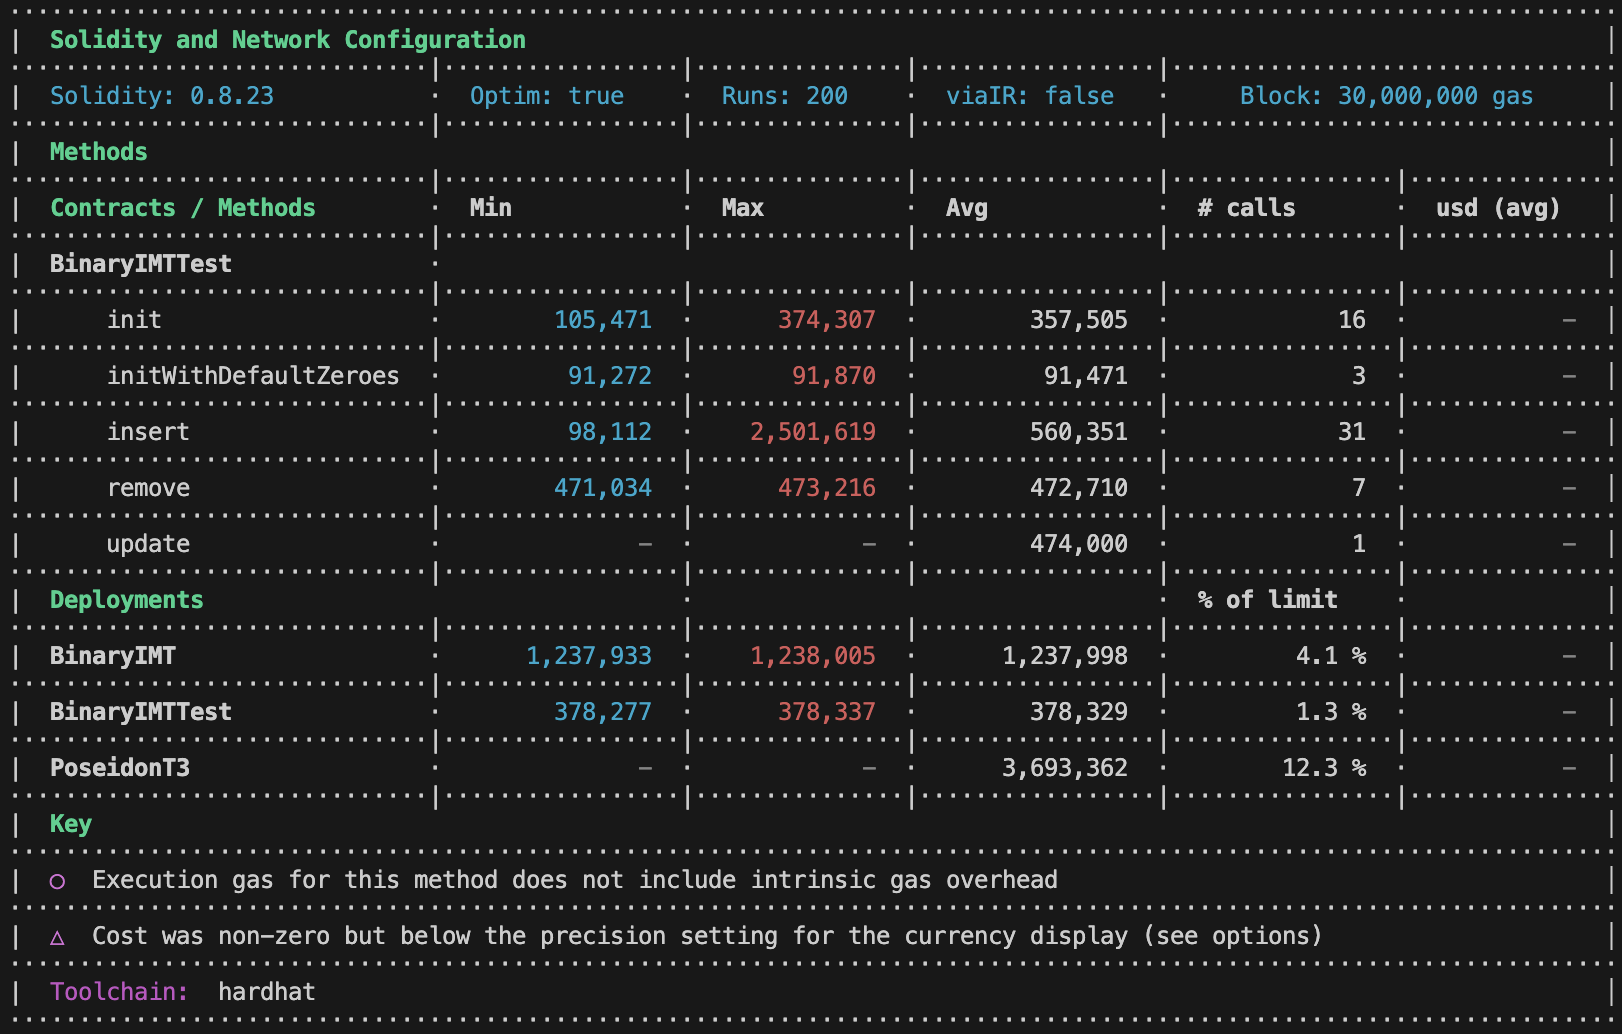
\includegraphics[width=\textwidth]{images/imt-gas-report.png}
    \caption{IMT Gas Report}
    \label{fig:imt-gas-report}
\end{figure}

\begin{figure}[H]
    \centering
    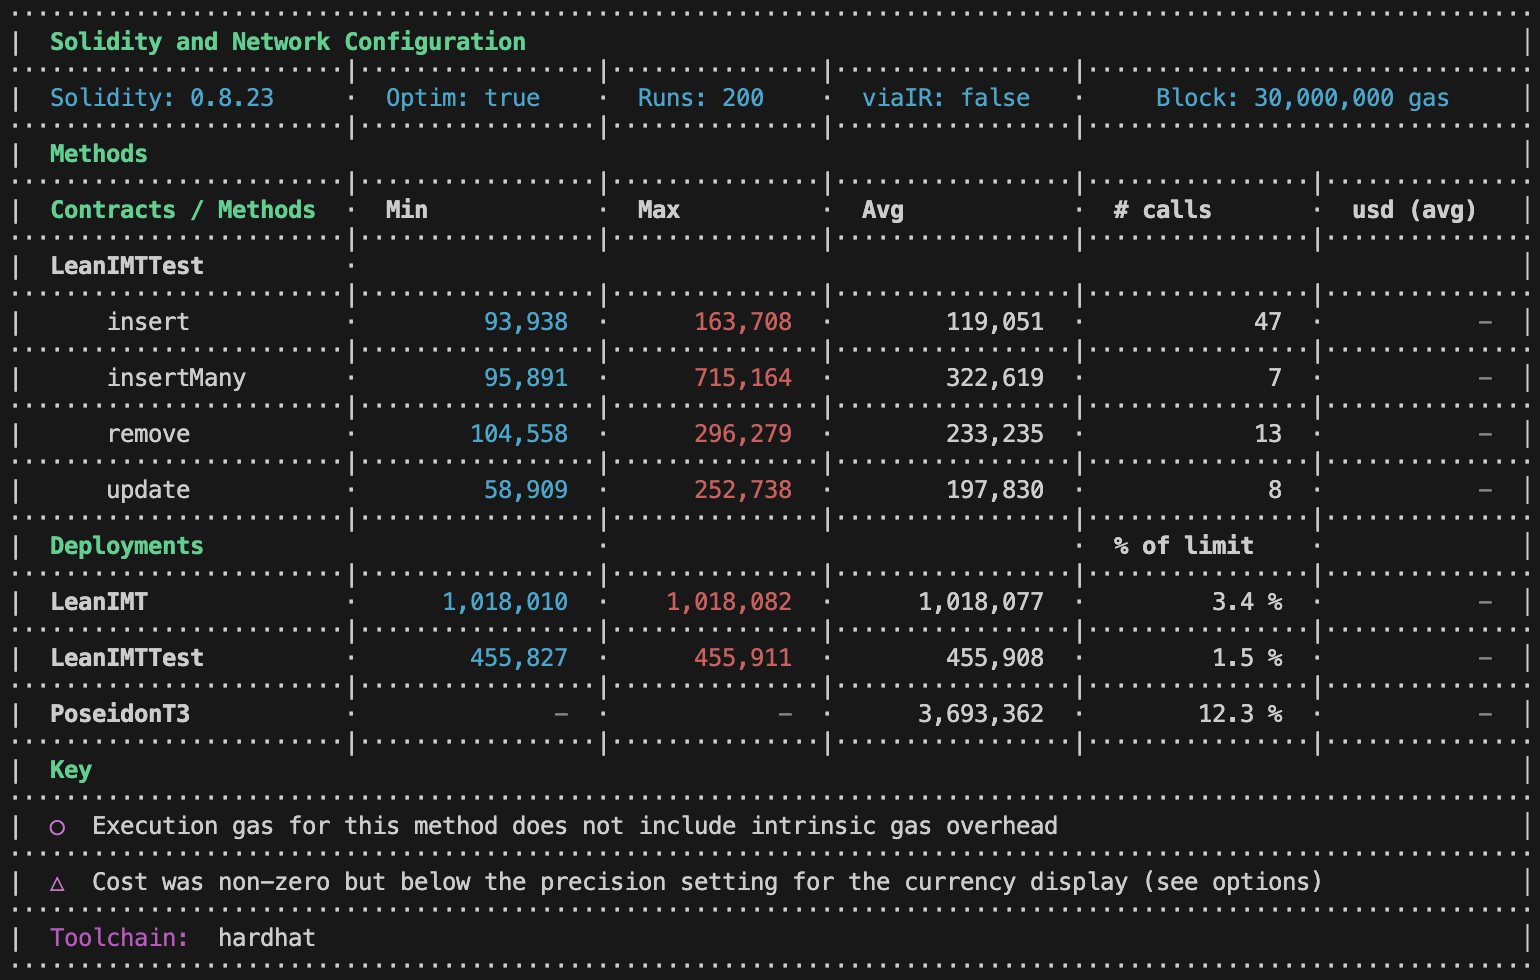
\includegraphics[width=\textwidth]{images/leanimt-gas-report.png}
    \caption{LeanIMT Gas Report}
    \label{fig:leanimt-gas-report}
\end{figure}

% Bar chart

\begin{figure}[H]
    \centering
    \pgfplotstableread[col sep=comma,]{data/gas-cost-functions-bar.csv}\datatable
    \begin{tikzpicture}
        \begin{axis}[
                ybar,
                xlabel={Function},
                xtick=data,
                xticklabels from table={\datatable}{Function},
                ylabel={Average Units of gas},
                ymin=0, % Set y-axis minimum to 0
                grid=major, % Add grid
                enlargelimits=0.15,
                legend style={at={(1.05,1)}, anchor=north west}, % Position the legend outside the plot
                legend cell align={left}, % Align legend text to the left
                % nodes near coords,
                xticklabel style={rotate=45, anchor=east} % Rotate x-axis labels
            ]
            \addplot[color=blue600, fill=blue400] table [x expr=\coordindex, y={IMT}, col sep=comma]{\datatable};
            \addlegendentry{IMT}

            \addplot[color=green600, fill=green400] table [x expr=\coordindex, y={LeanIMT}, col sep=comma]{\datatable};
            \addlegendentry{LeanIMT}
        \end{axis}
    \end{tikzpicture}
    \caption{Gas cost of the execution of the Functions IMT vs LeanIMT}
    \label{fig:gas-price-functions-bar}
\end{figure}

\section{Conclusions}

This technical document explains the LeanIMT algorithms, proves their correctness and analyzes their time complexity. The benchmarks show the improvements of LeanIMT, which is the data structure used in Semaphore v4, over the IMT used in Semaphore v3.

\subsection{Future Work}

As future work, a function to update many members at once (similar to the \textit{insertMany} function to insert many members at once) will be developed. Additionally, a Rust implementation of the data structure will be created to benchmark the performance in Node.js and browser environments.

% Allow LaTeX to break lines more flexibly in the bibliography
\sloppy

% Bibliography section
\printbibliography

% This is the end of the document
\end{document}